Use Root-Locus analysis to answer the questions about the following feedback control system 
\begin{center}
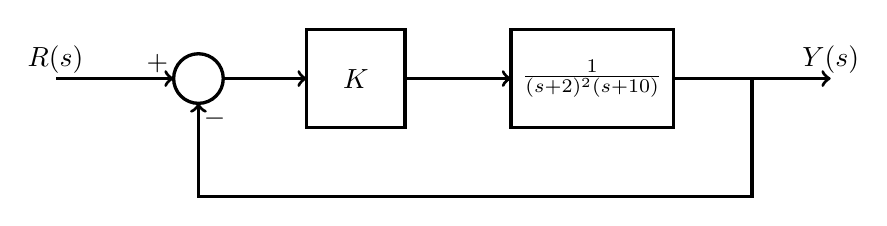
\begin{tikzpicture}[scale=1,inner sep=0pt,outer sep=0pt,very thick,
sysblock/.style={draw,rectangle,inner sep=4pt,minimum width=1.25cm,minimum height=1.25cm,very thick}]

\draw (-2,0) node[draw,circle] (sum1) {$\rule{0pt}{18pt}$};
\draw (0,0) node[sysblock] (K)  {$K$};
\draw (3,0) node[sysblock] (G) {$\frac{1}{(s+2)^2(s+10)}$};
\draw[<-] (sum1.180) node[above left=2pt] {$+$} -- ++(-1.5,0) node[above=2pt] {$R(s)$};
\draw[->] (sum1.0) -- (K.180);
\draw[->] (K.0) -- (G.180);
\draw[->] (G.0) --  ++(2,0) node[above=2pt] {$Y(s)$};
\draw[->] (G.0) -- ++(1,0) -- ++(0,-1.5) -| (sum1.-90) node[below right=2pt] {$-$};
\end{tikzpicture}
\end{center}

\begin{enumerate}[(a)]
\item Sketch the root locus for this system.
\item Suppose the gain $K$ is slowly increased. Using the asymptotes, estimate the frequency at which the step response will oscillate as the closed loop system goes from stable to unstable. 
\item Find the gain $K$ at which the system goes unstable (say, using Routh Hurwitz). 
\item Using \textsc{Matlab} find the step response for a slightly smaller value of $K$, and check your answer to part (b).
\end{enumerate}
